\documentclass[aspectratio=43]{beamer}
\usefonttheme[onlymath]{serif}
\usepackage[latin1]{inputenc}
\usepackage{tikz}
\usepackage{xcolor}
\usepackage{amsmath,amssymb,epsfig,graphicx,url,bbm,epstopdf}
\usepackage{graphicx}

%\usetheme{Szeged}
\useoutertheme[subsection=false, footline=institutetitle]{miniframes}
\usecolortheme{beaver}
\usepackage{media9}

\newcommand{\btVFill}{\vskip0pt plus 1filll}

\setbeamercolor{subtitle}{fg=black} % Change subtitle color
\setbeamercolor{block title}{fg=black} % Change subtitle color
\setbeamercolor{itemize item}{fg=black}
\setbeamercolor{enumerate item}{fg=black}
\setbeamercolor{itemize subitem}{fg=black}
\setbeamercolor{itemize itemize}{fg=red}

\setbeamertemplate{navigation symbols}{}%remove navigation symbols
\definecolor{darkgreen}{rgb}{0,0.5,0}

% Footer
\makeatletter
\setbeamertemplate{footline}
{
	\leavevmode%
	\hbox{%
		\begin{beamercolorbox}[wd=.333333\paperwidth,ht=2.25ex,dp=1ex,left]{section in head/foot}%
			\usebeamerfont{author in head/foot}\insertshortauthor
		\end{beamercolorbox}%
		\begin{beamercolorbox}[wd=.333333\paperwidth,ht=2.25ex,dp=1ex,center]{section in head/foot}%
			\usebeamerfont{title in head/foot}\insertshorttitle
		\end{beamercolorbox}%
		\begin{beamercolorbox}[wd=.333333\paperwidth,ht=2.25ex,dp=1ex,right]{section in head/foot}%
			\usebeamerfont{date in head/foot}\insertshortdate{}\hspace*{2em}
			\insertframenumber{} / \inserttotalframenumber\hspace*{2ex} 
		\end{beamercolorbox}}%
		\vskip0pt%
	}
	\makeatother
	
	\setbeamertemplate{caption}{\raggedright\insertcaption\par} % Removes the word "Figure" from captions
	
	\usebackgroundtemplate{	\tikz\node[opacity=0.03] {\includegraphics[height=500px,width=500px]{stanford_seal.png}}; }
	
	% Removes title background bar
	\setbeamercolor*{frametitle}{bg=}
	\setbeamercolor{titlelike}{parent=structure}
	
	\title[Stanford University]{Globally-Optimal Greedy Algorithms for Tracking a Variable Number of Objects}
	\subtitle{\scriptsize \vspace{3mm}Hamed Pirsiavash, Deva Ramanan, and Charless C. Fowlkes\\University of California, Irvine\vspace{-3mm}}
	\author[\enspace\,\,\, Albert Haque, Fahim Dalvi]{
		{\scriptsize Presented By}\\
		{\small Albert Haque and Fahim Dalvi}\\
		\vspace{-6mm}}
	\institute[Stanford University]{}
	\date{April 29, 2015}
	
	
	\begin{document}
		
		\section{}% Top left running header
		\begin{frame}
			\titlepage
		\end{frame}
		
		\begin{frame}{Outline}
			\begin{itemize}
				\item Motivation \& Related Work
				\item Mathematical Representation
				\begin{itemize}
					\item Probabilistic Framework
					\item ILP Formulation
				\end{itemize}
				\item Multiple Object Tracking
				\begin{itemize}
					\item Globally Optimal Greedy Algorithm
					\item Approximate Dynamic Programming Algorithm
				\end{itemize}
				\item Experiments and Results
			\end{itemize}
		\end{frame}
		
		\begin{frame}{Motivation}
			\begin{itemize}
				\item Single object tracking isn't enough
				\item In reality, multiple objects appear and occlusion is present
			\end{itemize}
			\begin{figure}
				\centering
				\includegraphics[width=0.5\linewidth]{figures/pull_new.png}
			\end{figure}
		\end{frame}
		
		
		\begin{frame}{Problem Statement}
			\begin{itemize}
				\item Input: a video sequence with bounding boxes
				\item Output: assignment of IDs to all tracks
				\item Representation: a point $x$ in \textit{spacetime}
				\begin{itemize}
					\item $x$ includes pixel location, scale, time frame
				\end{itemize}
			\end{itemize}
			\begin{center}
				\includemedia[
				activate=pageopen,
				width=200pt,height=120pt,
				addresource=video.mp4,
				flashvars={%
					source=video.mp4% same path as in addresource!
					%   &autoPlay=true%    % optional configuration
					%   &loop=true%        % variables
				}  
				]{}{VPlayer.swf}
			\end{center}
			\vfill
			{\fontsize{4}{12} \selectfont 
				Open in Adobe Reader to view in-slide video \\ \vspace{-2.7mm}
				Source: Jodoin, J. \textit{et al.} Urban Tracker: Multiple Object Tracking in Urban Mixed Traffic. Applications of Computer Vision. 2014.
			}
		\end{frame}
		
		\begin{frame}{How can we solve multi-object tracking?}
			\vspace{3mm}
			\uncover<2->{
				\scriptsize Answer: stitch together individual tracklets
				\begin{itemize}
					\item\scriptsize  Examples: trajectory prediction, flow-networks, matching
				\end{itemize}
				\vspace{-6mm}
			}
			\vfill
				\begin{columns}
					\uncover<3->{
						\column{.33\textwidth}
						\centering
						\begin{figure}
							\caption{\centering\tiny Track estimation with temporal trajectories $[1]$}
							\includegraphics[width=0.8\textwidth]{figures/related_work/silvio.png}
						\end{figure}
					}
					\uncover<4->{
						\column{.33\textwidth}
						\centering
						\begin{figure}
							\centering
							\caption{\centering\tiny Joint modeling of trajectory groupings $[2]$}
							\includegraphics[width=0.8\textwidth]{figures/related_work/pellegrini_joint_model_trajectories.png}
						\end{figure}
					}
					\uncover<5->{
						\column{.33\textwidth}
						\centering
						\begin{figure}
							\centering
							\caption{\centering\tiny Forecasting with Social Affinity Map (SAM) descriptors $[3]$}
							\includegraphics[width=0.43\textwidth]{figures/related_work/alex.png}
						\end{figure}
					}
				\end{columns}
				\uncover<6->{
					\vspace{5mm}
					Limitations:
					\begin{itemize}
						\item Fails when objects move unpredictably (e.g. sports)
					\end{itemize}
				}
				\vspace{5mm}
				{\fontsize{4}{12} \selectfont
					\uncover<3->{$[1]$ W. Choi and S. Savarese. Multiple target tracking in world coordinate with single, minimally calibrated camera. ECCV, 2010.\\ \vspace{-1.8mm}}
					\uncover<4->{$[2]$ S. Pellegrini, A. Ess, and L. Gool. Improving data association by joint modeling of pedestrian trajectories and groupings. ECCV, 2010.\\ \vspace{-1mm}}
					\uncover<5->{$[3]$ A. Alahi, V. Ramanathan, and L. Fei-Fei. Socially-aware large-scale crowd forecasting. CVPR, 2014.}
				}
		\end{frame}
		
		\begin{frame}{How can we solve multi-object tracking?}
			\begin{columns}
				\column{1\textwidth}
				\vspace{4mm}
				\centering
				{\scriptsize Hungarian bipartite graph matching [4, 5]}
				\vspace{-7mm}
				\begin{figure}
					\centering
					\includegraphics[width=0.7\linewidth]{figures/related_work/rowan_hungarian_bipartite.png}
				\end{figure}
				
			\end{columns}
			\uncover<2->{
				\vspace{5mm}
				Limitations:
				\begin{itemize}
					\item Is locally optimal but not globally optimal across time
				\end{itemize}
			}
			\vfill
			{\fontsize{4}{12} \selectfont
				$[4]$ H. Kuhn, \textit{et al.} The Hungarian method for the assignment problem. 1993. \\ \vspace{-2mm}
				$[5]$ M. Rowan and F. Maire. An efficient multiple object vision tracking system using bipartite graph matching. 2004.
			}
		\end{frame}
		
		\begin{frame}{How can we find the globally optimal solution?}
			\uncover<2->{
				\footnotesize
				Answer: Integer linear programs (ILP)
				\begin{itemize}
					\item Restrict possible locations to a finite set of candidate windows
				\end{itemize}
			}
			\vspace{-7mm}
			\uncover<3->{
				\begin{columns}
					\column{.6\textwidth}
					\centering
					\begin{figure}
						\centering
						\caption{\tiny LP-approach to multiple tracking [6]}
						\includegraphics[width=1.0\textwidth]{figures/related_work/jiang_lp_for_tracking.png}
					\end{figure}
					
					\column{.4\textwidth}
					\centering
					\vspace{2mm}
					\begin{figure}
						\centering
						\caption{\tiny Integer programming approach [7]}
						\includegraphics[width=.9\textwidth]{figures/related_work/andriyenko_lattice.png}
					\end{figure}
				\end{columns}
			}
			\vspace{3mm}
			\footnotesize
			\uncover<4->{
				Limitations:
				\begin{itemize}
					\item Doesn't scale well
					\item Limited or no occlusion modeling % (e.g. can produce broken tracks)
				\end{itemize}
			}
			\vfill
			\uncover<3->{
				{\fontsize{4}{12} \selectfont
					$[6]$ H. Jiang. \textit{et al.} A linear programming approach for multiple object tracking. CVPR, 2007. \\ \vspace{-1mm}
					$[7]$ A. Andriyenko and S. Konrad. Globally optimal multi-target tracking on a hexagonal lattice. ECCV, 2010.
				}
			}
		\end{frame}
		
		\begin{frame}{Contributions}
			\only<1>{
				\small
				Past attempts require \textbf{prior information} while some methods are \textbf{not globally optimal}. Linear programs are optimal but \textbf{not efficient}.
			}
			\only<2>{
				This paper proposes an ILP tracking formulation that:
				\begin{itemize}
					\item is globally optimal
					\item is locally greedy
					\item scales linearly in the number of objects
					\item scales quasi-linearly in the number of frames
				\end{itemize}
			}
		\end{frame}
		
		\begin{frame}{Research Questions}
			\begin{itemize}
				\item How can we represent tracking as a probabilistic framework?
				\item How can we formulate this as an ILP?
				\item How can we efficiently solve it?
				\item How can we guarantee optimality?
			\end{itemize}
		\end{frame}
		
		
		\begin{frame}{Algorithm Pipeline}
			\begin{columns}
				\column{0.33\textwidth}
				\uncover<1->{
					\begin{figure}
						\includegraphics[width=\textwidth]{figures/pipeline/1_new.eps}
					\end{figure}
				}
				\column{0.33\textwidth}
				\uncover<2->{
					\begin{figure}
						\includegraphics[width=\textwidth]{figures/pipeline/2_new.eps}
					\end{figure}
				}
				\column{0.33\textwidth}
				\uncover<3->{
					\begin{figure}
						\includegraphics[width=\textwidth]{figures/pipeline/3_new.eps}
					\end{figure}
				}
			\end{columns}
			\begin{columns}
				\column{0.17\textwidth}
				\column{0.33\textwidth}
				\uncover<4->{
					\begin{figure}
						\includegraphics[width=\textwidth]{figures/pipeline/4_new.eps}
					\end{figure}
				}
				\column{0.33\textwidth}
				\uncover<5->{
					\begin{figure}
						\includegraphics[width=\textwidth]{figures/pipeline/5_new.eps}
					\end{figure}
				}
				\column{0.17\textwidth}
			\end{columns}
		\end{frame}
		
		%%%%%%%%%%%%% OUTLINE
		\begin{frame}{Outline}
			\begin{itemize}
				{\color{gray}
					\item Motivation \& Related Work
				}
				\item Mathematical Representation
				\begin{itemize}
					\item Probabilistic Framework
					\item ILP Formulation
				\end{itemize}
				{\color{gray}
					\item Multiple Object Tracking
					\begin{itemize}
						{\color{gray}
							\item Globally Optimal Greedy Algorithm
							\item Approximate Dynamic Programming Algorithm
						}
					\end{itemize}
					\item Experiments and Results
				}
			\end{itemize}
		\end{frame}
		
		
		
		
		\begin{frame}{Notation}
			We define a state vector $x$ (i.e. a point in \textit{spacetime}):
			$$ x = (p, \sigma, t) \textrm{\quad and \quad} x \in V $$
			Where:
			\begin{itemize}
				\item $p=$ pixel location
				\item $\sigma =$ scale factor
				\item $t=$  frame number
				\item $V=$ set of all spacetime points
			\end{itemize}
			\vspace{5mm}
			A track $T$ is a set of state vectors: $ T = \{x_1,...,x_N\} $  \\
			Let $X$ denote a set of $K$ tracks: $ X = \{T_1, ..., T_K\} $
		\end{frame}
		
		\begin{frame}{Hidden Markov Model}
			Let $X$ denote the output tracking assignments:
			\begin{equation}
			P(X) = \prod_{T \in X} P(T)
			\end{equation}
			\uncover<2->{
				\begin{equation}
				P(T) = P_s(x_1) \left( \prod_{n=1}^{N-1} P(x_{n+1} | x_n) \right) P_t(x_N)
				\end{equation}
				Where:
				\begin{itemize}
					\item $P_s(x_1)$ is the prior for a track starting at $x_1$
					\item $\prod_{n=1}^{N-1} P(x_{n+1} | x_n) $ is the probability we follow some track
					\item $P_t(x_N)$ is the prior for a track ending at $x_N$
				\end{itemize}
			}
		\end{frame}
		
		\begin{frame}{Modeling Occlusion}
			To model occlusion:
			\begin{itemize}
				\item Allow tracks to be composed of non-consecutive frames
			\end{itemize}
			\only<1>{
				\begin{figure}
					\centering
					\includegraphics[width=0.8\textwidth]{figures/occlusion/blank.eps}
				\end{figure}
			}
			\only<2>{
				\begin{figure}
					\centering
					\includegraphics[width=0.8\textwidth]{figures/occlusion/not_occluded.eps}
				\end{figure}
			}
			\only<3->{
				\begin{figure}
					\centering
					\includegraphics[width=0.8\textwidth]{figures/occlusion/occluded.eps}
				\end{figure}
			}
			\color{white}
			{\only<4->{\color{black}}
				Note: $P(x_{n+1}|x_n)$ does not refer to the next frame but rather the next spacetime location in the track
			}
		\end{frame}
		
		\begin{frame}{MAP Inference}
			\uncover<1->{
				\begin{itemize}
					{\small
						\item $Y=$ all features $y_i$ observed at all spacetime points $i \in V$ in a video
						\item Goal: Select $X^*$ such that it maximizes the likelihood of $Y$
					}
				\end{itemize}
			}
			\uncover<2->{
				\begin{align}
				X^* &= \underset{X}{\mathrm{argmax \; }} P(X)P(Y|X)  \\
				&=  \underset{X}{\mathrm{argmax }} \prod_{T \in X} P(T) \prod_{x \in T} l(y_x)  \\
				&=  \underset{X}{\mathrm{argmax }} \sum_{T \in X} \log P(T) + \sum_{x \in T} \log l(y_x)
				\color{white}
				\end{align}
				
				\begin{itemize}
					\item where $ l(y_x) = \frac{P_{\textrm{FG}}(y_x)}{P_{\textrm{BG}}(y_x)} $ and $P_{\textrm{FG}}, P_{\textrm{BG}} \sim \mathcal{N}$
				\end{itemize}
			}
		\end{frame}
		
		\begin{frame}{How can we find the MAP?}
			\uncover<2->{Answer: Represent MAP as an integer linear program (ILP)}
			\begin{itemize}
				\item \uncover<3->{Let $i,j$ be different frames}
				\item \uncover<4->{$ f_{ij}, f_i, f_i^s, f_i^t $ are indicator variables}
				\item \uncover<5->{$c_i^s = -\log P_s(x_i) \quad c_i^t = - \log P_t(x_i) $}
				\item \uncover<6->{$c_{ij} = - \log P(x_j | x_i)$}
				\item \uncover<7->{$c_i = - \log l(y_i)$}
			\end{itemize}
		\end{frame}
		
		\begin{frame}{How can we find the MAP?}
			Formal ILP definition:
			\begin{align}
			\onslide<2->{ f^* &= \underset{x}{\mathrm{argmin \; }} C(f) \\ }
			\onslide<3->{ \textrm{ with } C(f) &=  {\only<7->{\color{blue}}\sum_{i} c_i^s f_i^s } + {\only<7->{\color{blue}} \sum_{ij \in E} c_{ij} f_{ij} } + {\only<7->{\color{red}} \sum_{i} c_i f_i } + {\only<7->{\color{blue}} \sum_{i} c_i^t f_i^t } \\ }
			\onslide<4->{ \mathrm{ s.t. \quad} & f_{ij}, f_i, f_i^s, f_i^t \in [0,1] \\ }
			\onslide<5->{ \mathrm{ and \quad} & f_i^s + \sum_i f_{ji} = f_i = f_i^t + \sum_j f_{ij} \\ }
			\onslide<6->{ \mathrm{ and \quad} & \sum_i f^t_i = K \\}
			\notag
			\end{align}
			\vfill
			\tiny{Where $E$ is the set of permissible state transitions given by dynamic model}
		\end{frame}
		
		
		%\begin{frame}{How can we solve the ILP?}
		%\begin{itemize}
		%\item Answer: Represent ILP as a network / use network flow to solve
		%\item Relax the problem such that $f's$ are now real valued
		%\begin{itemize}
		%\item Fortunately the conversion leads to a network flow problem with \textit{totally unimodular} constraints, which means the optimal solution will still be integral
		%\end{itemize}
		%\item Find K min-cost flows as:
		%\end{itemize}
		%\begin{center}
		%\small{MAP estimate for K tracks $\equiv$ Pushing a flow of K through the graph}
		%\end{center}
		%\end{frame}
		
		\begin{frame}{How can we solve the ILP?}
			\only<2->{ 
				\begin{itemize}
					\item Answer: Represent ILP as a network-flow problem
				\end{itemize}
				\vspace{-5mm}
			}
			\only<2>{
				\begin{figure}
					\centering
					\includegraphics[width=1\textwidth]{figures/network_model.eps}
				\end{figure}
			}
			\only<3>{ 
				\begin{figure}
					\centering
					\includegraphics[width=1\textwidth]{figures/network_model_labeled.eps}
				\end{figure}
			}
			\vspace{-6mm}
			\color{white}
			{\only<3->{\color{black}}
				\centering\scriptsize{$c_i^s = -\log P_s(x_i) \quad\; c_i^t = - \log P_t(x_i) \quad\; c_{ij} = - \log P(x_j | x_i) \quad\; c_i = - \log l(y_i)$}
			}
		\end{frame}
		
		\begin{frame}{Outline}
			\begin{itemize}
				{\color{gray}
					\item Motivation \& Related Work
					\item Mathematical Representation
				}
				\begin{itemize}
					{\color{gray}
						\item Probabilistic Framework
						\item ILP Formulation
					}
				\end{itemize}
				\item Multiple Object Tracking
				\begin{itemize}
					\item Globally Optimal Greedy Algorithm
					\item Approximate Dynamic Programming Algorithm
				\end{itemize}
				{\color{gray}
					\item Experiments and Results
				}
			\end{itemize}
		\end{frame}
		
		
		\begin{frame}{How can we find the min-cost flows?}
			\begin{itemize}
				\item Answer: Push a flow of $K$ through the graph
				\item \uncover<2->{ Using properties of our network:}
				\begin{itemize}
					\item \uncover<2->{All edges are unit capacity}
					\item \uncover<2->{Network is a DAG}
				\end{itemize}
				\item \uncover<3->{Best previous method $[8,9]$: $O(N^3 \log N)$ }
				\item \uncover<4->{We achieve a $O(KN \log N)$ algorithm}
			\end{itemize}
			\vfill
			{\fontsize{4}{12} \selectfont
				$[8]$ L. Zhang \textit{et al.} Global data association for multi-object tracking using network flows. CVPR, 2008.  \\ \vspace{-2mm}
				$[9]$ A. Goldberg. An efficient implementation of scaling minimum-cost flow algorithm. Journal of Algorithms, 1997.
			}
			\smallskip
		\end{frame}
		
		
		\begin{frame}{How can we find the min-cost flows?}
			This paper proposes three algorithms:
			\begin{itemize}
				\item Successive shortest-paths
				\item Approximate One-Pass DP for $K>1$
				\item Approximate Two-Pass DP for $K>1$
			\end{itemize}
		\end{frame}
		
		\begin{frame}{Successive Shortest Paths}
			\only<1>{
				\begin{figure}
					\centering
					\includegraphics[width=1.0\textwidth]{figures/ssp/ssp1.png}
				\end{figure}
			}
			\only<2>{
				\begin{figure}
					\centering
					\includegraphics[width=1.0\textwidth]{figures/ssp/ssp2.png}
				\end{figure}
			}
			\only<3>{
				\begin{figure}
					\centering
					\includegraphics[width=1.0\textwidth]{figures/ssp/ssp3.png}
				\end{figure}
			}
			\only<4>{
				\begin{figure}
					\centering
					\includegraphics[width=1.0\textwidth]{figures/ssp/ssp4.png}
				\end{figure}
			}
			\only<5>{
				\begin{figure}
					\centering
					\includegraphics[width=1.0\textwidth]{figures/ssp/ssp5.png}
				\end{figure}
			}
			\only<6>{
				\begin{figure}
					\centering
					\includegraphics[width=1.0\textwidth]{figures/ssp/ssp6.png}
				\end{figure}
			}
		\end{frame}
		
		
		\begin{frame}{Successive Shortest Paths}
			\begin{itemize}
				\item Problem: Using residual graph introduces negative flows
				\item \uncover<2->{Solution: Convert residual graph to positive costs only}
				\begin{itemize}
					\item \uncover<2->{Requires computing shortest path from source to all nodes}
					\item \uncover<2->{$O(N^2)$ with Bellman-Ford}
				\end{itemize}
				\item \uncover<3->{Our DP approach: $O(N)$}
			\end{itemize}
		\end{frame}
		
		%		\begin{frame}{How to speed up conversion?}
		%			\begin{itemize}
		%				%\item Problem: Usual methods of converting a graph with negative edge weights to one without them are slow
		%				%\item Solution: Use the fact that the original graph is a DAG
		%				\item Dynamic Programming Approach that runs in O(N)
		%			\end{itemize}
		%		\end{frame}
		
		\begin{frame}{Dynamic Programming Approach}
			\only<1>{
				\begin{figure}
					\centering
					\includegraphics[width=1.0\textwidth]{figures/dp/1.eps}
				\end{figure}
				\begin{center}
					Start with a partial ordering of the nodes based on time
					
					\color{white} {
						$\pi = \underset{j \in N(i)} \min c_{ij} + cost(j)$
					}
				\end{center}
			}
			\only<2>{
				\begin{figure}
					\centering
					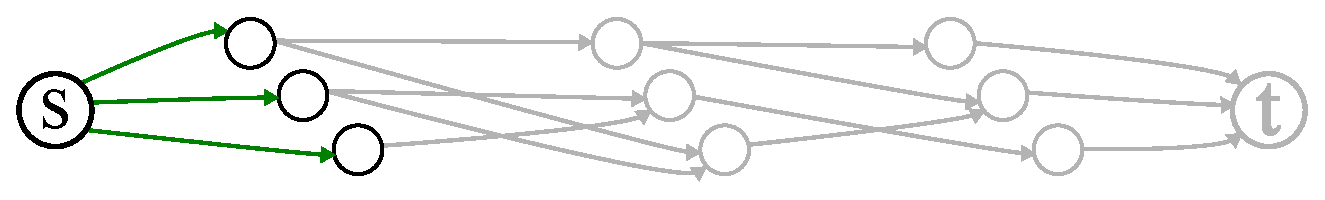
\includegraphics[width=1.0\textwidth]{figures/dp/2.eps}
				\end{figure}
				\begin{center}
					$cost(i)=c_i + c_i^s$
					
					\color{white} {
						$\pi = \underset{j \in N(i)} \min c_{ij} + cost(j)$
					}
				\end{center}
			}
			\only<3>{
				\begin{figure}
					\centering
					\includegraphics[width=1.0\textwidth]{figures/dp/3.eps}
				\end{figure}
				\begin{center}
					$cost(i)=c_i + \min(\pi, c_i^s)$
					
					$\pi = \underset{j \in N(i)} \min c_{ij} + cost(j)$
				\end{center}
			}
			\only<4>{
				\begin{figure}
					\centering
					\includegraphics[width=1.0\textwidth]{figures/dp/4.eps}
				\end{figure}
				\begin{center}
					$cost(i)=c_i + \min(\pi, c_i^s)$
					
					$\pi = \underset{j \in N(i)} \min c_{ij} + cost(j)$
				\end{center}
			}
			\only<5>{
				\begin{figure}
					\centering
					\includegraphics[width=1.0\textwidth]{figures/dp/5.eps}
				\end{figure}
				\begin{center}
					$cost(i)=c_i + \min(\pi, c_i^s)$
					
					$\pi = \underset{j \in N(i)} \min c_{ij} + cost(j)$
				\end{center}
			}
			\only<6>{
				\begin{figure}
					\centering
					\includegraphics[width=1.0\textwidth]{figures/dp/6.eps}
				\end{figure}
				\begin{center}
					$cost(i)=c_i + \min(\pi, c_i^s)$
					
					$\pi = \underset{j \in N(i)} \min c_{ij} + cost(j)$
				\end{center}
			}
			\only<7>{
				\begin{figure}
					\centering
					\includegraphics[width=1.0\textwidth]{figures/dp/7.eps}
				\end{figure}
				\begin{center}
					$cost(i)=c_i + \min(\pi, c_i^s)$
					
					$\pi = \underset{j \in N(i)} \min c_{ij} + cost(j)$
				\end{center}
			}
		\end{frame}
		
		
		\begin{frame}{How can we track one object?}
			\begin{itemize}
				\item \uncover<2->{Shortest path corresponds to optimal solution for $K=1$}
				\item \uncover<3->{Conversion algorithm gives us shortest path from source node to terminal node}
			\end{itemize}
		\end{frame}
		
		\begin{frame}{How can we track multiple objects?}
			Approximate One-Pass DP $O(KN)$ Algorithm:
			\begin{itemize}
				\item \uncover<2->{ Start with original flow graph, perform $K+1$ iterations: }
				\begin{itemize}
					\item \uncover<3->{Find shortest path from $s$ to $t$}
					\item \uncover<4->{If path cost is negative, remove nodes on the path}
				\end{itemize}
				\item \uncover<5->{At each iteration, we instance one track}
				%\item Suboptimal because each successive iteration works on a subset of the original graph nodes
				%\item But shown to work well in practice
			\end{itemize}
		\end{frame}
		
		\begin{frame}{Outline}
			\begin{itemize}
				{\color{gray}
					\item Motivation \& Related Work
					\item Mathematical Representation
				}
				\begin{itemize}
					{\color{gray}
						\item Probabilistic Framework
						\item ILP Formulation
					}
				\end{itemize}
				{\color{gray} \item Multiple Object Tracking }
				\begin{itemize}
					{\color{gray}
						\item Globally Optimal Greedy Algorithm
						\item Approximate Dynamic Programming Algorithm
					}
				\end{itemize}
				\item Experiments and Results
			\end{itemize}
		\end{frame}
		
		\begin{frame}{Datasets}
			\footnotesize
			\begin{itemize}
				\item Caltech Pedestrian Dataset [7]: 71 videos, 1800 frames each, 30 fps \\
			\end{itemize}
			\vspace{-3mm}
			\begin{figure}
				\centering
				\includegraphics[width=0.9\textwidth]{figures/experiments/caltech.png}
			\end{figure}
			\begin{itemize}
				\item ETHMS Dataset [8]: 4 videos, 1000 frames each, 14 fps
			\end{itemize}
			\vspace{-3mm}
			\begin{figure}
				\centering
				\includegraphics[width=0.3\textwidth]{figures/experiments/ethms.jpg}
			\end{figure}
			
			
			{\fontsize{4}{12} \selectfont
				$[7]$ Dollar, P. \textit{et al.} Pedestrian detection: A benchmark. CVPR, 2009. \\ \vspace{-1mm}
				$[8]$ Ess, A. \textit{et al.} A Mobile Vision System for Robust Multi-Person Tracking. CVPR, 2008.
			}
			
		\end{frame}
		
		\begin{frame}{Evaluation Metrics}
			\footnotesize
			\uncover<2->{
				$$ \textrm{Detection rate (recall)} = \frac{\textrm{Number of correct ID labelings}}{\textrm{Total number of ID labelings}} $$
				\\ \vspace{5mm}
			}
			\uncover<3->{
				$$ \textrm{False positives per image (FPPI)} = \frac{\textrm{Total number of false positives}}{\textrm{Number of images (frames)}} $$
				\\ \vspace{5mm}
			}
			\uncover<4->{
				$$ \textrm{Identification error} = \frac{\textrm{Number of incorrect ID labelings}}{\textrm{Total number of ID labelings}} $$
			}
		\end{frame}
		
		
		\begin{frame}{Detection Rate vs False Positives per Image (FPPI)}
			\begin{figure}
				\centering
				\includegraphics[width=0.8\linewidth]{figures/experiments/detection_vs_fppi.png}
			\end{figure}
			\uncover<2->{
				Key Insights:
				\begin{itemize}
					{\small
						\item SSP produces short tracks due to 1st order Markov property
						\item DP produces longer tracks because tracks are never cut or edited
					}
				\end{itemize}
			}
		\end{frame}
		
		\begin{frame}{Track Label Error vs Allowed Occlusion}
			\begin{table}
				\centering\footnotesize
				\caption{Results on ETHMS Dataset (Ideal Detector)}
				\begin{tabular}{cc}
					\hline
					Length of Allowable Occlusion & Windows with ID Errors \\ \hline
					1 & 14.69\% \\
					5 & 13.32\% \\
					10 & 9.39\% \\ \hline
				\end{tabular}
			\end{table}
			Key Insight:
			\begin{itemize}
				\item Larger occlusion windows improve performance
			\end{itemize}
		\end{frame}
		
		
		\begin{frame}{Performance Comparison}
			
			\begin{table}
				\footnotesize\centering
				\begin{tabular}{lcc}
					\hline
					Algorithm & Detection Rate & FPPI \\ \hline
					Stereo Algorithm $[10]$ & 47.0 & 1.50 \\ 
					MAP/Min-Cost Flow $[11]$ & 68.3 & 0.85 \\ 
					MAP/Min-Cost Flow + Occlusion Handling $[11]$ & 70.4 & 0.97 \\ 
					Two-Stage + Occlusion Handling $[12]$ & 75.2 & 0.93 \\ 
					\textbf{Our DP} & \textbf{76.6} & \textbf{0.85} \\
					\textbf{Our DP + NMS} & \textbf{79.8} & \textbf{0.85} \\ \hline
				\end{tabular}
			\end{table}
			\vfill
			{\fontsize{4}{12} \selectfont
				$[10]$ A. Ess \textit{et al.} Depth and appearance for mobile scene analysis. ICCV, 2007. \\ \vspace{-1.5mm}
				
				$[11]$ L. Zhang \textit{et al.} Global data association for multi-object tracking using network flows. CVPR, 2008.  \\ \vspace{-2mm}
				
				$[12]$ J. Xing \textit{et al.} Multi-object tracking through occlusions by local tracklets filtering and global tracklets association. CVPR, 2009.
			}
		\end{frame}
		
		
		\begin{frame}{Cost versus iteration number}
			\begin{itemize}
				\item DP algorithm is close to optimal (SSP) while being orders of magnitude faster
			\end{itemize}
			\begin{figure}
				\centering
				\includegraphics[width=0.6\linewidth]{figures/experiments/cost_vs_iteration.png}
			\end{figure}
		\end{frame}
		
		\begin{frame}{Algorithm Runtime}
			\begin{itemize}
				\item DP algorithm is two orders of magnitude faster than commercial solvers
			\end{itemize}
			\begin{figure}
				\centering
				\includegraphics[width=0.75\linewidth]{figures/experiments/runtime.eps}
			\end{figure}
		\end{frame}
		
%						\item 
%						\item How can we formulate this as an ILP?
%						\item How can we efficiently solve it?
%						\item How can we guarantee optimality?
%		
		\begin{frame}{Conclusion}
			\only<1>{
				Given the input, we answered several research questions:
				\begin{figure}
					\includegraphics[width=0.6\textwidth]{figures/pipeline/1_new.eps}
				\end{figure}
			}
			\only<2>{
				How can we represent tracking as a probabilistic framework?
				\begin{figure}
					\includegraphics[width=0.6\textwidth]{figures/pipeline/2_new.eps}
				\end{figure}
			}
			\only<3>{
				How can we formulate this as an ILP?
				\begin{figure}
					\includegraphics[width=0.6\textwidth]{figures/pipeline/3_new.eps}
				\end{figure}
			}
			\only<4>{
				How can we efficiently solve it?
				\begin{figure}
					\includegraphics[width=0.6\textwidth]{figures/pipeline/4_new.eps}
				\end{figure}
			}
			\only<5>{
				This allowed us solve the multi-object tracking problem:
				\begin{figure}
					\includegraphics[width=0.6\textwidth]{figures/pipeline/5_new.eps}
				\end{figure}
			}
		\end{frame}	
					
		
		%		\begin{frame}{Conclusion}
		%			
		%			\setbeamercolor{itemize item}{fg=gray}
		%			\setbeamercolor{itemize subitem}{fg=gray}
		%			
		%			{\only<3->{\color{gray}} How can we represent tracking as a probabilistic framework? } 
		%			\begin{itemize}
		%				\item \uncover<2->{ {\only<3->{\color{gray}} Use a hidden Markov model and MAP estimate } }
		%			\end{itemize}
		%			\vspace{3mm}
		%			{\only<4->{\color{gray}}  How can we formulate this as an optimization problem? }
		%			\begin{itemize}
		%				\item \uncover<3->{ {\only<4->{\color{gray}} With integer linear programming } }
		%			\end{itemize}
		%			\vspace{3mm}
		%			{\only<5->{\color{gray}}  How can we efficiently solve this optimization problem? }
		%			\begin{itemize}
		%				\item \uncover<4->{ {\only<5->{\color{gray}} Formulate ILP as a graph, use min-flow, and DP } }
		%			\end{itemize}
		%			\vspace{3mm}
		%			How can we guarantee optimality? 
		%			\begin{itemize}
		%				\item \uncover<5->{ Successive shortest path algorithm } 
		%			\end{itemize}
		%		\end{frame}
		
		
		\begin{frame}{}
			\centering
			\vfill
			\huge Questions?
			\vfill
		\end{frame}
		
	\end{document}